\documentclass[letterpaper, 11pt]{article}


%=================================================

\usepackage{fullpage, parskip}
\usepackage{fancyhdr}	%% Header and footer
\usepackage{amsmath, mathtools}
\usepackage{amssymb}	%% mathbb, \ll
%\usepackage{esint}	%% surface integral symbol
\usepackage[round,authoryear]{natbib}	% Citations
%\usepackage{gensymb, upgreek}
\usepackage{ulem}	%% Underline matrices
\usepackage[breaklinks,backref,bookmarks=true]{hyperref}
\usepackage{enumitem}	%% Resume numbering in enumerate
%\usepackage{varioref}	%% \vref -- says where target is
\usepackage{url}
\usepackage{graphicx}
%\usepackage{caption}
\usepackage{subcaption}
\captionsetup{compatibility=false}
\usepackage[usenames,dvipsnames]{color}
\usepackage{pdfpages}
\usepackage{xspace}	%% Guesses whether to put space after command
%\usepackage{attachfile}	%% Attach multimedia files
%\usepackage{listings} %% Include source code
\usepackage{aas_macros} %% Journal control sequences

%--------------------------------------------------
%% Header and Footer
\pagestyle{fancy}
\fancyhead{}
\renewcommand{\headrulewidth}{0.0pt}
\rfoot{Cato Sandford}
\lfoot{Summer 2012}
%%--------------------------------------------------
\def\kB{\ensuremath{k_{\rm B}}\xspace}
\def\psfobs{\ensuremath{{\rm PSF_{obs}}}\xspace}
\def\psfref{\ensuremath{{\rm PSF_{ref}}}\xspace}
%%--------------------------------------------------
%% Language macros
\def\etc{{\&c.}\xspace}	% Not italicised
\def\th{\textsuperscript{th}\xspace}
\def\ra{\ensuremath{\rightarrow}\xspace}
%%--------------------------------------------------
%% Editing Macros
\def\wspace{\textcolor{white}{Lorem ipsum}}
\def\TODO#1{ {\color{red}{\bf TODO: {#1}}}\xspace}
\def\MORE{{\color{red}{\bf MORE}}\xspace}
\def\REF{{\color{OliveGreen}{\bf REF}}\xspace}
%%=================================================


%% Top matter
\title{Report\\}
\author{Cato Sandford\thanks{Department of Physics, New York University, USA; \texttt{cato@nyu.edu}}}
\date{\today}

%%-------------------------------------------------

\begin{document}

\maketitle

\wspace\newline\wspace\newline


\begin{abstract}
A sketch of my project with DWH and PJM: image deconvolution and colour-composition.
\end{abstract}


\begin{center}
\line(1,0){250}
\end{center}
\vspace{-0.5cm}
\tableofcontents
\vspace{-0.1cm}
\begin{center}
\line(1,0){250}
\end{center}
\newpage


%%=================================================
%% Introduction
%%=================================================
\section{Introduction}

\begin{quote}
	I found I could say things with color and shapes that I couldn't say any other way -- things I had no words for.\\	
	\mbox{}~\hfill -- Georgia O'Keeffe
\end{quote}

Astronomers continue to astonish the world with images of a Universe far richer and more magnificent than any ordinary eye could perceive or any mind conceive. Indeed, astronomy has always depended heavily on images\MORE

\begin{itemize}
	\item Sophistication of modern analysis
	\item 
	\item The big picture: lens zoo, image presentation and combination.
\end{itemize}


PHIL: `Basically we want to make PS1, DES, HSC and LSST data as informative
as possible for astronomers who want to *look at images*. My own
interest is in finding gravitational lenses, but basically anyone who
wants to see what they have found in the object catalog database
should be interested in this work.'

\subsection{The Point-Spread Function (PSF)}

\subsection{Bandpasses and Colour Images}

\newpage
%%=================================================
%% DECONVOLUTION
%%=================================================
\section{Deconvolution}
\label{sec:deconvolution}

As mentioned in the introduction, it is frequently possible and indeed desirable to reduce or control the bluriness of a telescope image. In this section, we describe how one might do this -- the procedure is as follows:

\begin{enumerate}
	\item Identify the astronomical sources in a FITS image.
	\item Find the point sources, and from these estimate the PSF of the image. We call this the ``observed PSF'', or \psfobs.\label{pnt:getpsf}
	\item Generate a symmetrical\footnote{Well, not actually circularly symmetric.} target PSF for the image, using the dimensions and flux properties of the image PSF of point~\ref{pnt:getpsf}. We call this the ``reference PSF'' or \psfref.\label{pnt:PSF0}
	\item Create an object which maps the observed PSF to the reference PSF. This object is called the ``kernel'' and the mapping procedure is convolution.
	\item Apply this procedure to the original image; this should correlate all the pixels in such a way as to rid the image of asymmetrical blurriness and replace it with a blurriness of known properties.
\end{enumerate}

The reader may be confused at this point as to why, if we can correctly calculate the PSF of an image, we don't simply do away with the blurriness altogether -- i.e. find a kernel which maps the PSF to a point. This would be a ``hard deconvolution'', a procedure which is compellingly discouraged by the work of \cite{MCS98} (see appendix~\ref{sec:MCS98notes} for more discussion of this paper). Following this work, we may endeavour to obtain better knowledge of the sky by reducing the PSF, but we must avoid inadvertently violating the sampling theorem, which would certainly happen if we attempted a hard deconvolution.

Once we have made the target PSF as small as possible within this restriction, we can enforce that it be symmetrical uniform throughout the whole image: this is a ``soft deconvolution''. The result of this will be that all point sources have the same pre-determined shape, and extended sources will be superpositions of this shape.

Mathematically, we can think of \psfobs as being composed of the reference PSF convolved with a messy 2D function $K$:
\begin{align}
	\psfobs(\vec x) = \psfref(\vec x) \ast K(\vec x).
	\intertext{In the following sections, we discuss how we determine the observed PSF, construct the reference PSF, and find the convolution kernel $K$. Crucially for homogenising the image, we must also find the kernel $k$ which governs the inverse transformation, i.e.}
	\psfobs(\vec x) \ast k(\vec x) = \psfref(\vec x).
\end{align}


%%=================================================
%% SExtractor
%%=================================================
\subsection{Source Identification}
\label{sec:sextractor}




\begin{itemize}
	\item Use SExtractor to identify the sources in an image
	\item How does it work?
	\item What else does it measure / output?
\end{itemize}

\wspace

\begin{itemize}
	\item SExtractor reads in a FITS image and catalogues all the astronomical sources it contains.
	\item My code automates this by generating catalogues of an entire directory of images, using some special settings.
	\item These default settings are (mostly) in the files \texttt{prepsfex.sex} (governs how the program runs) and \texttt{prepsex.param} (governs what information about the sources is recorded in the output file).
	\item The program outputs a file with extension \texttt{.cat} (by default, if the image is called \texttt{image.fits}, the output will be \texttt{image.cat}). This contains information like the position, elongation and flux of the source.
\end{itemize}

%%=================================================
%% PSFEx
%%=================================================
\subsection{Determining the PSF of an Image}
\label{sec:psfex}

\begin{itemize}
	\item Use PSFEx to compute \psfobs (arbitrary shape, noisy)
	\item How does it work? Use that graph in the docs.
	\item What else does it measure / output?
\end{itemize}

\wspace

\begin{itemize}
	\item PSFEx uses the \texttt{.cat} file from SExtractor, and estimates the PSF in the image.
	\item There are a considerable number of options for how this estimation is done and what form the outputs take. After flirting with some of the more sophisticated options, it turns out that the key thing for my purpose is an integrated image of the average PSF for the image. This is saved as FITS.
	\item I have automated the PSFEx step to process all the image catalogues in a directory with some default settings imposed (these are kept in \texttt{default.psfex}).
\end{itemize}

%%=================================================
%% PSF Generation
%%=================================================
\subsection{Generating an Idealised PSF}

\begin{itemize}
	\item Find moments of PSFEx \psfobs (2D)
	\item Find total flux
	\item Size of PSF image
	\item Plug into a 2D Gaussian 
	\item Generate FITS files
\end{itemize}

Some comments on generating 

\begin{itemize}
	\item We wish to deconvolve the image such that it has a constant, symmetrical PSF of finite width.
	\item My code reads in the FITS file containing the PSF; it calculates the total flux, and the width of the PSF in the $y$ and $x$ directions. Then it generates the image of a 2D Gaussian which shares these properties. This is the ``ideal'' PSF.
\end{itemize}

%%=================================================
%% Kernel
%%=================================================
\subsection{Mapping to the Target PSF, \psfref}
\label{sec:kernel}


Find the convolution kernels which map between these two versions of the PSF.
\begin{itemize}
	\item In order to deconvolve the entire image to the reference PSF, we must find an object which, when convolved with the \psfobs gives \psfref. This object is the convolution kernel, which is we retrieve by casting the deconvolution procedure as a linear algebra problem.
\end{itemize}
\wspace\newline\wspace\newline

Say we have two similar images: $\mathcal{A}$, which is a picture taken by a real telescope, and $\mathcal{B}$ which is the same image but deconvolved to a constant, ideal PSF $r(\vec x)$. We need to deconvolve the image  $\mathcal{A}$ by some kernel $k$ in order to leave $\mathcal{B}$ with a clean PSF of $\psfref(\vec x)$. Since convolution is a linear operation, we can cast our search for the convolution kernel in terms of a linear algebra problem. Specifically, we want to solve (for $\vec k$) an equation of the form
\begin{equation}\label{eqn:vector}
	\vec b = A \vec k,
\end{equation}
where $A$ and $\vec b$ encode the original and deconvolved image, and $\vec k$ represents the convolution kernel (also an image). When written in this form, our problem of finding $\vec k$ becomes a traditional vector-equation--solve.

The vectors $\vec b$ and $\vec k$ are easy to construct -- just flatten the respective images. If $\mathcal B$ is an image of $n\times m$ pixels, then $\vec b$ will have $nm$ elements. $A$ is less strightforward, and we must think carefully about the convolution process to understand what's going on here.

\MORE

$A$ is then a matrix with ${\rm size}(b)$ rows and ${\rm size}(k)$ columns. The vector problem in equation~\ref{eqn:vector} is overdetermined, so we must use some optimisation procedure (typically least-squares minimisation) to find $\vec k$.


\subsubsection{Interlude: Honesty Note}
\label{sec:shave}

When we convolve two images, we produce a new image pixel by taking a weighted sum of the surrounding pixels. For instance, say we convolve a large image $\mathcal{A}$ with a 3$\times$3-pixel image to get $\mathcal{B}$. The first (i.e. top-left) pixel of $\mathcal{B}$ that we can properly determine is not the same as the first pixel of $\mathcal{A}$, because \MORE.

Thus, the honest thing to do is to throw away some information by making image $\mathcal B$ smaller than $\mathcal A$ -- in this example with a 3$\times$3 image, we shave off the four outer edges, so if $\mathcal A$ is $N\times M$, $\mathcal B$ is $(N-2)\times(M-2)$. A bigger convolving image would require more pixels to be lost from the result.

This contrasts with the traditional solution to the problem, which is to ``pad'' the original image with zeroes (see figure~\ref{fig:zeropad}) such that the final image is the same size as the (pre-padded) original was. This seems to introduce spurious information -- how can we possibly know that there are zeros at the border of an image? Often this is patently not the case, even for astronomical images which can be mostly black. With this in mind, it may seem preferable to adopt the ``lossy'' procedure outlined in the last paragraph.

DWH has argued semi-convincingly that we needn't make such a sacrifice in practice, because there is enough information in the border pixels to mitigate grave data-fabrication. Hmm\ldots

\begin{figure}[h]\label{fig:zeropad}
	\centering
	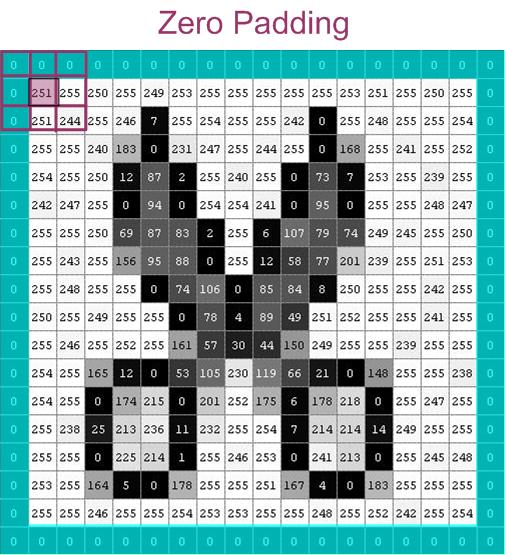
\includegraphics[width=0.33\linewidth]{Images/pad_zero_color.jpg}
	\caption{An image padded with zeroes. Convolution with the 3$\times$3 stencil will now preserve image size; but at what cost?}
\end{figure}



%%=================================================
%% Deconvolution
%%=================================================
\subsection{Full Image Deconvolution}

In section~\ref{sec:kernel} we found the kernel $k$ which would transform a messy PSF image into a nice symmetrical one with known properties (\psfobs $\rightarrow$ \psfref.). This same kernel can be used to transform an entire image with the observed PSF, $\mathcal C$, into the same image\footnote{Modulo concerns raised in section~\ref{sec:shave}.} with the target PSF, $\mathcal D$. To do this, we must perform the operation
\begin{align}
	\mathcal{D} = k \ast \mathcal{C},
	\shortintertext{or, in the language of linear algebra,}
	\vec{d} = \uuline{K} \vec{c}.\label{eqn:convolve}
\end{align}
The image vectors $\vec d$ and $\vec c$ have the same form as discussed earlier -- they are simply flattened versions of the pixel-arrays. The kernel matrix $\uuline K$ is more tricky; but after some refelxion, it transpires that $\uuline K$ is a sparse, upper-diagonal matrix where every row is identical, but shifted right by one element with respect to the row above. (Note that in practice it is unweildy and prohibitively expensive to store all the zero-entries of the $\uuline K$ matrix -- we have to be a little bit clever about how to store and manipulate the relevant information.)

Once we have constructed an appropriate kernel matrix and multiplied it by the (observed) image vector, we are done.

Alternatively, we can simply use a pre-existing module which performs the convolution for us: \texttt{scipy.signal.fftconvolve} does the job nicely. We can even tell this module to reduce the size of the convolved image (\texttt{mode="valid"}).

However, it would be naive to simply place our trust in SciPy -- their convolution method may be subtly different from the one we wish to use for scientific inference. Thus, we cannot escape having to implement the concolution procedure of equation~\ref{eqn:convolve}. Figure~\ref{fig:deconvolution_comparison} shows a comparison, with residuals. Leaving aside the image artefacts from using a small convolution kernel (\MORE FIX!), we can see that the two methods do not agree completely. This is worrying, but according to DWH the problem is almost certainly with my implementation rather than SciPy's, and I am inclined to agree (it might be a simple indexing error). Combined with the fact that SciPy is around 15 times faster, it makes little sense to labour on with my code; so we adopt the SciPy convolution module.

\begin{figure}
	\def\width{0.3\textwidth}
	\centering
	\begin{subfigure}{\width}
		\includegraphics[width=\textwidth]{../Data/Deconvolved/gsc_CFHTLS_03_g_sci_rescaled.png}
		\caption{Original image}
	\end{subfigure}
	
	\begin{subfigure}{\width}
		\includegraphics[width=\textwidth]{../Data/Deconvolved/gsc_CFHTLS_03_g_sci_rescaled_MAN.png}
		\caption{Deconvolved using my procedure and a 3x3 kernel.}
	\end{subfigure}
	~
	\begin{subfigure}{\width}
		\includegraphics[width=\textwidth]{../Data/Deconvolved/gsc_CFHTLS_03_g_sci_rescaled_SCI.png}
		\caption{Deconvolved using SciPy's procedure and a 3x3 kernel.}
	\end{subfigure}
	
	\begin{subfigure}{\width}
		\includegraphics[width=\textwidth]{../Data/Deconvolved/gsc_CFHTLS_03_g_sci_rescaled_RES.png}
		\caption{Residuals.}
	\end{subfigure}
	\caption{Deconvolution procedure -- a comparison of my home-made convolution algorithm and SciPy's optimised one. SciPy takes about 1/15 of the time. Note that a 3x3 kernel was used for this test, and there are obvious artefacts introduced around bright points of the image.}
	\label{fig:deconvolution_comparison}
\end{figure}


%%=================================================
%% Test Noise Properties
%%=================================================
\subsection{Noise Properties}

Here I've applied a few different stretches to the original image and to the deconvolved image. The left-hand side images are all stretched originals and the right-hand side are all stretched deconvolutions. The stertch gets more sever as you go down.


Specific notes:\\
* I used a 9x9 kernel for these images.\\
* To change the strength of the stretch, I simply divided the upper bound (you called it "vmax") by 2 and 10.\\

\includepdf[pages={1,2}]{../Data/Deconvolved/CFHTLS_03_g_Deconvolved_noisecompare.pdf}


%%=================================================
%% Image Manipulation
%%=================================================
\subsection{Image Manipulations}

\begin{itemize}
	\item Making them viewable by humans -- stretch
	\item .psf file conversion
	\item FITS conversion
\end{itemize}




%%=================================================
%% RBG
%%=================================================
\section{Colour Combination}

Telescope data is often given in ``bands'' -- we do not record the total flux coming from a point in the sky, but the flux in a certain wavelength range. This information allows us to investigate the properties of astronomical objects, such as temperature and chemical composition. However to make a readily-interprable image which contains maximum information in one hit, we need to combine the bands to make a colour-composite image.

Many methods had been developed to do this in accordance with researchers' individual aesthetic preference. But the full richness of possibility was still unexploited, until \citet{Lup++04} demonstrated just how much detail one could extract from data when colour was given its deserved treatment (see appendix~\ref{sec:Lup++04notes} for more detail). Using their method, we can combine images from different bands in a way which enhances hidden or faint features without allowing bright objects to dominate. It has the further advantage that the brightness of an object in the image is decoupled from its colour. The method is implemented in PJM's \emph{HumVI} (formerly \emph{ColorJPG}).

A further improvement to the method was implemented by Wherry (\MORE describe difference
\footnote{PHIL: `My reading of it is that Lupton uses two parameters, Q and alpha, to
tweak the look of the image, while Wherry's IDL code takes 4 input
parameters: 3 image scales and a nonlinearity parameter.
I like Wherry's approach because I *think* I want to make images that
all have the same scales and limits, that is, that a pixel of a
particular colour and brightness in field1.png is representing the
same set of surface brightnesses that a pixel of equal colour and
brightness is in field2.png. I want to develop intuition about the
objects, and the noise level, through displaying a lot of images! Note
that display of noise is itself an issue - I am unlikely to want to
use your "kill noise" option, but am happy for the zero surface
brightness level in the image to be dark grey instead of black.

Anupreeta More has made a very nice set of test CFHTLS images for the
Lens Zoo, and I discussed with her a bit your work: she thinks we
should do a blind taste test at some point, showing the lens zoo dev
team her images that have been a) displayed in standard form with
HumVI and b) deconvolved and then
displayed in standard form with HumVI, and ask for them to be graded
for arc visibility. Probably we would want to supply a few different
standard forms as well (and by "form" I mean {scales,nlin}). We can
also do image testing at Adler Planetarium on the willing public
there. The question we want to answer is: "how should we display an
image to maximize the likelihood of an untrained human seeing
interesting feature X?"  I have no idea where one sends paper like
this - Ill ask the zooniverse team.'}
). We translated Wherry's improvements from IDL to Python, and integrated this module with the HumVI code. Some additional improvements are also made, such as increased versatility with rebinning.

A summary of this part of the project (with pseudocode) follows.

\begin{enumerate}
	\item Translated (and improved?) the Wherry algorithm from IDL to Python (\texttt{wherry.py}). This is what it does:
	\texttt{
	\begin{enumerate}
		\item RGB = [readin(R\_data),readin(G\_data),readin(B\_data)]		\#\# *\_data can be filename, array of data, or a channel instance
		\item rescale(RGB, scalefactors)	\#\# multiply each band by a given number
		\item rebin(RGB, xrebinfactor,yrebinfactor)		\#\# re-sample images
		\item kill\_noise(RGB, cutoff)	\#\# sets all pixels below a threshold to 0
		\item arsinh\_stretch(RGB, nonlinearity)
		\begin{itemize}
			\item pixtot = R\_array+G\_array+B\_array	\#\# collapse images onto each other
			\item if pixtot[i,j]==0: pixtot[i,j]=1
			\item factor = arsinh(nonlin*rad)/(nonlin*rad)
			\item (R\_array,G\_array,B\_array) *= factor
		\end{itemize}
		\item if stauratetowhite==False: box\_scale(RGB)
		\begin{itemize}
			\item maxpixel[i,j] = max(R[i,j],G[i,j],B[i,j])	\#\# i.e. find the maximum pixel value of the three arrays
			\item if maxpixel[i,j] < 1: maxpixel[i,j]=1
			\item (R\_array,G\_array,B\_array) /= maxpixel
			\item (Also translates origin of image if required)
		\end{itemize}
		\item overlay/underlay \#\# not entirely sure what these are for
		\item scipy.misc.imsave(RGB)
	\end{enumerate}
	}
	\begin{itemize}
		\item Note: when treating \texttt{wherry.py} as a standalone code for making composite images, the user can choose which bands to use for R, G and B.
		\item Also, in the IDL version of the code, there is a function devoted to transforming the image data into bytes. When I was translating to Python, I found that this was an unnecessary IDL-specific step, and it was unnecessary to implement it.
	\end{itemize}
	\item Integrated with PJM's HumVI code, so that choice of Lupton/Wherry procedure is an option.
	\begin{itemize}
		\item Wherry is default. Luption can be invoked with command-line keyword \texttt{--lupton} or simply \texttt{-l}.
		\item Again, the user can choose which bands to use for R, G and B -- it just depends on the order of the three filenames.
		\begin{itemize}
			\item After some initial misunderstanding, I now use R=i, G=r, B=g.
		\end{itemize}
		\item Of course, this bands$\rightarrow$colour map is unchanged when when \texttt{--lupton} is specified.
	\end{itemize}
\end{enumerate}

%\begin{figure}
%  \centering
%    \includegraphics[width=\linewidth]{C:/Users/adam.BEYOND/Dropbox/Hogg_2012/Code/HumVI/images/test/CFHTLS_03_lw.pdf}
%  \caption{Restretched images and combination of three bands using two different procedures. \MORE specifics of algorithm / equation / pseudocode. \MORE crop.}
%\end{figure}




%%=================================================
%% UNMBRELLA
%%=================================================
\section{Combined Deconvolution and Colour}

Mag++98 -- must deconvolve all bands to target PSF before combining.


\newpage
%%=================================================
%% TO DO
%%=================================================
\section{To do}

\underline{Document}
\begin{itemize}
	\item Invert figure colours to save ink!\newline
	[Latex can't do this, I'll have to make them myself.]
\end{itemize}

\underline{Colour}
\begin{itemize}
	\item Make some side-by-side composites showing Wherry and Lupton
	\item Fail to compute scales $\rightarrow$ error
	\item Should work with one or two FITS images.
\end{itemize}

\underline{Deconvolution}
\begin{itemize}
	\item Use larger kernels
	\item Treat all three bands of a certain image with the same kernel -- should be the most conservative?
	\item User-specified PSF width. Keep total flux.
	\begin{itemize}
		\item Assert target PSFs of
width 0.3,0.4,0.5,0.6,0.7,0.8,0.9, 1.0 arcsec FWHM, and make deconvolved images for each value. Then plot your quality metric(s) against FWHM.
		\item When inventing metrics, consider that each one represents the quantitiave answer to a particular question about some aspect of the reconstructed image - its "noise" level, the correlated nature of that noise, the number of false SExtractor detections (in the reconstructed image) generated, the SExtractor flux of certain
objects of interest, the number of inspectors who identify feature X, etc etc etc. We can propose and discuss these aspects after seeing some images. These "aspects" could also be termed "failure modes"
	\end{itemize}
	\item Homogenise PSF across different fields. \TODO{What is the best way to do this?} Use largest PSF $\rightarrow$ no danger of violating sampling theorem; but this may be way too blurry to be useful. Pickle.
	\item PSFEx failure modes -- see Phil's e-mail.
	\item Propagate/append information in the original FITS header.
\end{itemize}

\underline{Combining C\&D}
\begin{itemize}
	\item Make pipeline for deconvolution to common \psfref then combination. (The deconvolution and colour composition procedures are not integrated into a pipeline. There are some small challenges in integrating them, but it shouldn't be too difficult. The main danger is that the code becomes too cumbersome and dependent on my directory structure.)
\end{itemize}

\underline{Maths}
\begin{itemize}
	\item PHIL: `I would like to see a derivation of this procedure, which involves a
matrix acting on a noisy vector. Do you start by writing down the
principled probabilistic inference of a model image given noisy data,
and end up showing that this boils down (under certain assumptions) to
the matrix operations you perform? Any improvements we make to your
code will probably be of the form "assign a different prior to the
pixel values of the kernel/final image", so it'd be good to see how
that propagates through into new matrix operations.'

	\item A prior on pixel values would lead to an
additional term (with a lagrange multiplier) added to the summed
squared residuals. It would be good to also include the weight image, that
characterises the actual per pixel uncertainty, because some pixels
are going to have very high uncertainty indeed... We need to be able
to cope with saturated pixels, chip gaps etc, and weight images is how
you do it, in general.
\end{itemize}




\newpage
%%=================================================
%% APPENDIX
%%=================================================
\appendix
\addcontentsline{toc}{section}{Appendix}
\section*{APPENDIX}

%%=================================================
%% MCS 1998 paper
%%=================================================
\section{Magain, Courbin \& Sohy 1998 -- ``Deconvolution with Correct Sampling''}
\label{sec:MCS98notes}

\paragraph{Key Ideas}

-- We shouldn't pretend to derive infinite resolution images from discrete data. A more honest approach can mitigate the appearance of 
artefacts.

-- Bear in mind that correlations in astrnomical images are local. Global treatments and techniques are inappropriate.


\paragraph{Background}

-- Ground-based telescopes suffer from aperture diffraction and from atmospheric inhomogeneities which distort light. One (post hoc) way of 
correcting for this is to infer the point spread function from a puative point source in your image; if we consider the data to represent 
"reality" or the "scene" convolved with this PSF, then we can in principle deconvolve the data from the PSF to retrieve the scene. 

-- There will be many scenes compatible with the (uncertain) data, so we must then pose the problem as an optimisation problem: we wish to 
find the scene, compatible with the data, that minimises some cost function to be devised. A typical procedure is to minimise the chi-squared 
function (between data and model).

-- Also want solution to be smooth, so introduce a Lagrange function which enforces this. A common procedure is to maximise the entropy of the 
image (using the flux distribution as the information). This has the benefit of requiring positive flux values.

-- So far we ignore noise in the image.

\paragraph{Problems}

-- Two problems emerge with this way of doing things: 1) often find image artefacts (from improper sampling, as we shall see); 2) it doesn't 
preserve the global intensity scale.

-- In practice, telescope cameras are constructed so that their data just satisfy the sampling theorem -- the pixel-spacing is ~2x the maximum 
frequency expected from objects. Upon deconvolution, where the fuzziness is taken out, the sampling theorem will be violated. Theoretically, 
deconvolution can introduce point-sources/Dirac-deltas (i.e. stars), so an infinitely small sampling interval would have to be used.

-- Deconvolution therefore leads to artefacts when there is a sharp discontinuity in the scene -- e.g. a star on a black background shows 
ringing. (Can think of this as a window in frequency space (i.e. a cutoff at some maximum frequency) leading to a sinc function in position-
space: the result of deconvolving a point source will be delta*sinc.)

-- In traditional methods, riniging is mitigated by the positivity 
constraint, which damps down the lobes of oscillations. But this depends crucially on the zero-level, and accurate subtraction of sky noise 
is necessary for the methods to wrok well.

-- Image artefacts steal flux and bias photometry. Also, maximising entropy makes the image as 
smooth (uniform) as possible, which tends to spread out point sources; peak intensity is thus undersetimated.


\paragraph{Proposal}

-- Do not do a full deconvolution: do a "light" deconvolution where point sources are given as extended objects of know size and flux 
distribution. These objects are chosen such that they satisfy the sampling theorems. In other words, reconstruct the image you would get if 
you had a better instrument (rather than a perfect instrument).

-- So now the image has a constant PSF, which M++ call r(x). This introduces a length scale over which the image must be smooth (?). This 
applies to point sources (which have shape r(x)) and extended sources. From the solution space of lightly-deconvolved scenes, we should 
choose the one which gives maximum smoothness on this local scale.

-- Specifically, for each pixel we take the difference of the "background" (everything which isn't delta) from the "reconstrcuted background" 
(the fixed PSF convolved with the scene); then sum over pixels and minimise (equation 7). This procedure discards high-frequecy information, 
but is consistent with the adopted sampling and the frequencies of r(x).

-- Artefacts not stealing flux AND no smoothing of point sources -> 
photometry possible.

-- Requires no positivity constraint.


\paragraph{Usage}

-- Using simulated and real astronomical images, with finite resolution and noise, the new procedure is compared with other standard 
procedures and does (stupidly) well. They are able to recover fluxes and positions to high accuracy, and they avoid exacerbating noise / 
artefacts in the image.

-- Image combination is also demonstrated -- deconvolution of many images to the same PSF before combining them yields 
high-resolution final image.


\paragraph{Further Work}

-- Devise a more robust optimisation that finds minimum even in populated images.


%%=================================================
%% Lupton et al. 2004 paper
%%=================================================
\section{Lupton et al. 2004 -- ``Preparing Red-Green-Blue Images from CCD Data''}
\label{sec:Lup++04notes}

- 'sheer drama and beauty of the night sky'

KEY IDEA
--------

- There is a lot of information in the colouration of an image. This often helps us distinguish features / phenomena and classify astronomical objects.

- Hitherto, focus has been on intensity differences.


BACKGROUND	
----------

- We apply stretches to images in order to coax faint objects into observability. But we must strike a balance between this objective and the saturation of bright parts.

- Stretch is a re-scale, bringing all objects to within a brightness cutoff range. Re-scale can be linear, ln, sqrt, depending on preference and the diversity of images.

- Tuning parameters is not always straightforward. Any object above maximum brightness ends up bleached and obese.

- Furthermore, there is degeneracy between brightness and colour in traditional stretching procedures.


SOLUTION
--------

- Using a different stretching procedure, (equation 2), can discard uninteresting intensity information in favour of colour information. This works by comparing the individual colour-intensities to the total intensity (i.e. ~ compare the colours amongst themselves), and comparing the total instensity to the two cutoff intensities which define the brightness scale.

- NB the colours are unique -- no degeneracy with intensity. So we can draw unambigouous conclusions from looking at colour differences.

- arsinh stretch magnifies faint objects (linear regime) and avoids bleaching bright objects (logarithmic regime). (But this could be achieved with other functions too).


EXAMPLES
--------

- Some examples are given where the standard technique loses an embarrassing amount of detail compared with the new idea. By eye, we clearly distinguish differences between objects which are otherwise just rendered as white blobs.


\newpage
\addcontentsline{toc}{section}{References}
\bibliographystyle{plainnat}
\bibliography{Hogg}

\end{document}
